%&"../net"
\endofdump
\tikzexternalize[prefix=cache/]{lab06}
\begin{document}
    \title{Overlay Network and VXLAN (With Bug)}
    \maketitle
    \tableofcontents
    \vfill
    An overlay network can be thought of as a computer network on top of another network. 

    VXLAN is often described as an overlay technology because it allows to stretch Layer 2 connections over an intervening Layer 3 network by encapsulating (tunneling) Ethernet frames in a VXLAN packet that includes IP addresses.
    \vfill
    \clearpage
    \section{建立网络}

    先克隆虚拟机\footnote{感谢 VMWare Workstation 的快照技术,如果重新启动虚拟机,网络配置将会让其无法上网,必须返回原点重新配置。},然后分别在 VM1 和 VM2 上分别运行 \href{run:vm1topo.py}{vm1topo.py} 和 \href{run:vm2topo.py}{vm2topo.py}(与 \verb"vm1topo.py" 类似,略过),得到如图 \ref{fig:toposym} 所示的拓扑结构,注意拓扑已经与教程中
    % 结果如图 \ref{fig:setup} 所示:

    % \code[language=bash]{vm1.sh}
    % \code[language=bash]{vm2.sh}

    \code{vm1topo.py}

    % \begin{figure}[H]
    %     \centering
    %     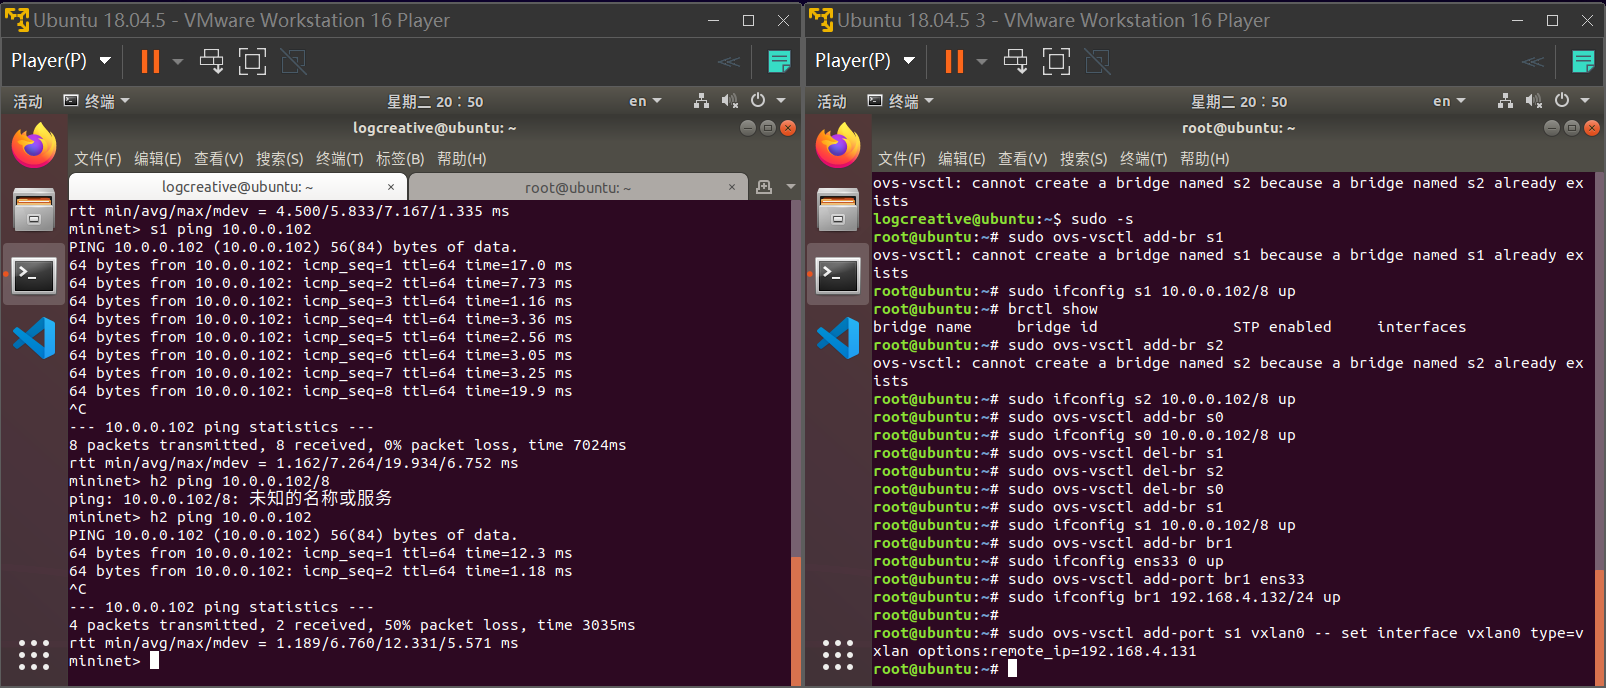
\includegraphics[width=\linewidth]{setup}
    %     \caption{配置环境}\label{fig:setup}
    % \end{figure}

    % \begin{figure}[H]
    %     \centering
    %     \begin{tikzpicture}
    \tikzstyle{host}=[draw]
    \tikzstyle{switch}=[draw]
    \tikzstyle{connection}=[]
    \tikzstyle{constr}=[right,font=\ttfamily\small]
    
\node (h1) [host] at (-0.5,0.5) {h1};
\node (s1) [switch] at (1.5,0.5) {s1};
\node (s3) [switch] at (3,2) {s3};
\node (s2) [switch] at (4.5,0.5) {s2};
\node (s4) [switch] at (3,-1) {s4};
\node (h2) [host] at (6.5,0.5) {h2};
\draw  (h1) edge (s1);
\draw  (s1) edge (s3);
\draw  (s3) edge (s2);
\draw  (s2) edge (s4);
\draw  (s4) edge (s1);
\draw  (s2) edge (h2);
\end{tikzpicture}
    %     \caption{拓扑结构}\label{fig:topo}
    % \end{figure}

    \begin{figure}[H]
        \centering
        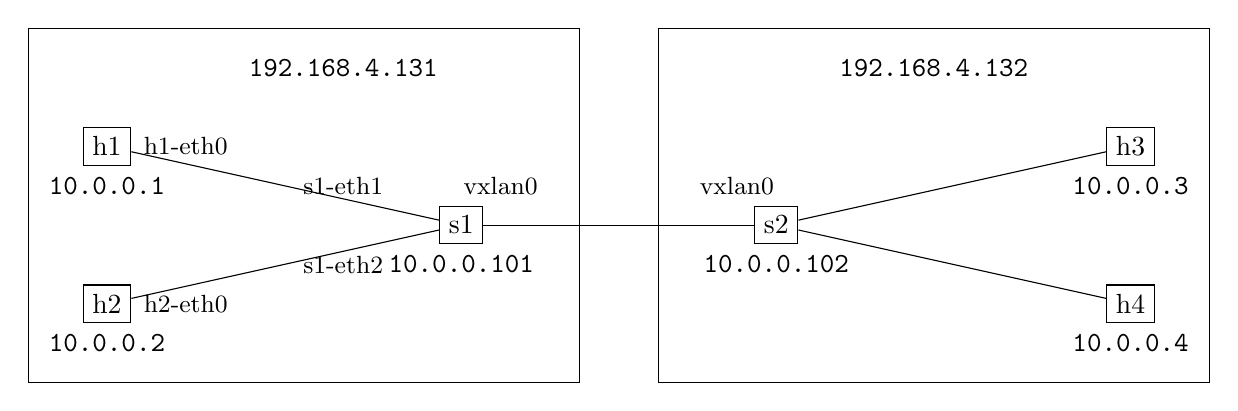
\begin{tikzpicture}[node distance=0.5cm]
\tikzstyle{host}=[draw]
\tikzstyle{switch}=[draw]
\tikzstyle{connection}=[]
\tikzstyle{constr}=[right,font=\ttfamily\small]
\draw  (-5,2) rectangle (2,-2.5);
\draw  (3,2) rectangle (10,-2.5);
\node [switch] (v2) at (0.5,-0.5) {s1};
\node [below of=v2,font=\ttfamily] {10.0.0.101};
\node [host] (v1) at (-4,0.5) {h1};
\node [below of=v1,font=\ttfamily] {10.0.0.1};
\node [host] (v3) at (-4,-1.5) {h2};
\node [below of=v3,font=\ttfamily] {10.0.0.2};
\draw  (v1) edge (v2);
\draw  (v3) edge (v2);
\node [host] (v4) at (4.5,-0.5) {s2};
\node [below of=v4,font=\ttfamily] {10.0.0.102};
\draw  (v2) edge (v4);
\node[font=\ttfamily] at (6.5,1.5) {192.168.4.132};
\node[font=\ttfamily] at (-1,1.5) {192.168.4.131};
\node[font=\small] at (4,0) {vxlan0};
\node[font=\small] at (1,0) {vxlan0};
\node[font=\small] at (-1,0) {s1-eth1};
\node[font=\small] at (-3,0.5) {h1-eth0};
\node[font=\small] at (-3,-1.5) {h2-eth0};
\node[font=\small] at (-1,-1) {s1-eth2};
\node [host] (v5) at (9,0.5) {h3};
\node [host] (v6) at (9,-1.5) {h4};
\draw  (v4) edge (v5);
\draw  (v4) edge (v6);
\node[below of=v5,font=\ttfamily] {10.0.0.3};
\node[below of=v6,font=\ttfamily] {10.0.0.4};
\end{tikzpicture}
        \caption{拓扑结构}\label{fig:toposym}
    \end{figure}

    \section{Wireshark 抓包}
    Use Wireshark to monitor the interfaces s1 and eth0, and describe your findings.

    使用 Wireshark 抓取传输时数据,得到如图 \ref{fig:wireshark} 所示的包。外层为 UDP 报文,显示的实际的 IP 地址;中间为 VXLAN 层;再内侧为 Overlay 的 ICMP 报文,显示的是 Overlay IP 地址。

    \begin{figure}[H]
        \centering
        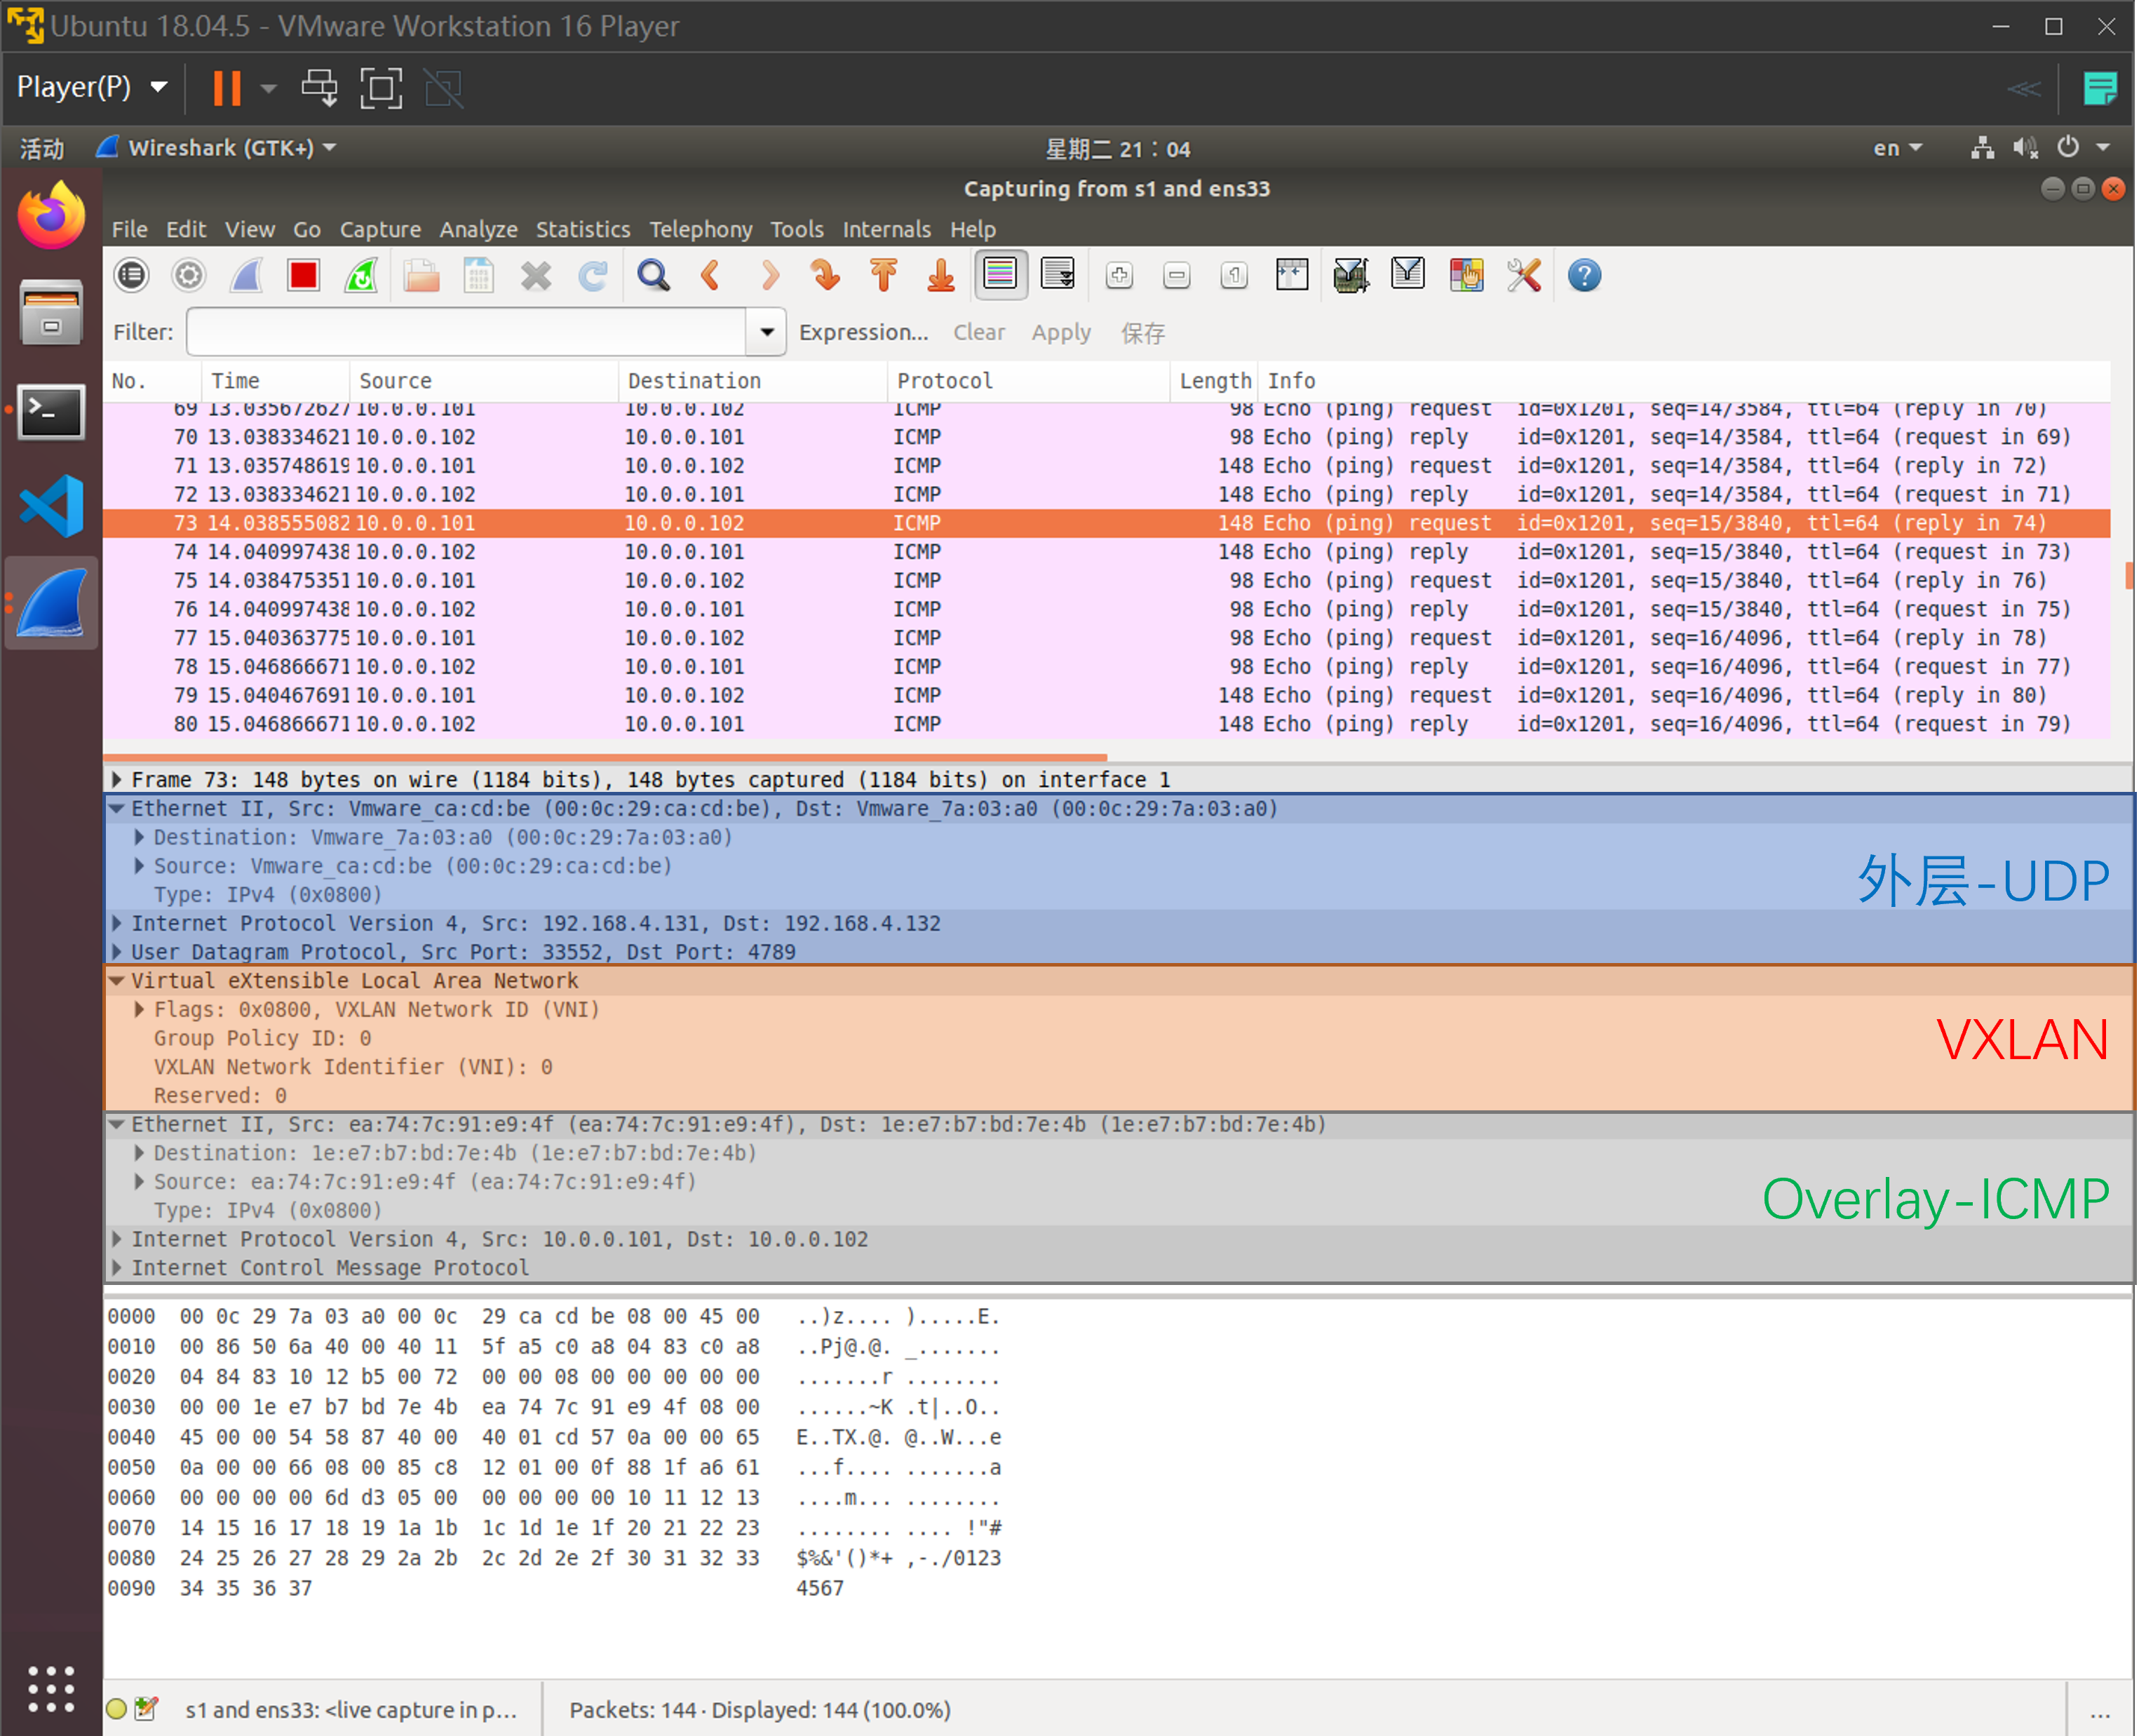
\includegraphics[width=\linewidth]{wireshark}
        \caption{Wireshark 抓包}\label{fig:wireshark}
    \end{figure}

    \section{iperf 测试}
    Use iperf to test the network bandwidth between the two virtual machines 
    \begin{itemize}
        \item Test the bandwidth between 192.168.56.127 and 192.168.56.128
        \item Test the bandwidth between 10.0.0.1/10.0.0.2/10.0.0.101 and 10.0.0.102 (hint: you may need to specify a reasonable MTU size in order for your iperf to work in this case. Please also think about why.)
    \end{itemize}

    Compare the above results and explain the reason. 

    % \begin{figure}[H]
    %     \centering
    %     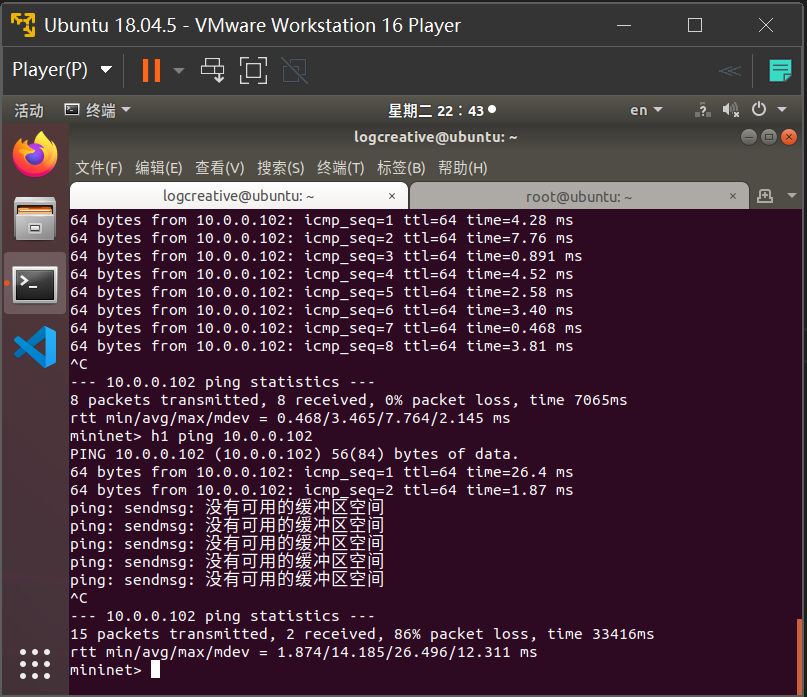
\includegraphics[width=0.7\linewidth]{nobuffer}
    %     \caption{没有可用的缓冲区空间}\label{fig:nobuffer}
    % \end{figure}

    % 使用控制器\cite{vxlannew}

    \section{ping 测试}
    Similar to Q2, use ping to test the network latency and analyze your results.

    如果不调整 MTU 会导致从 h1 ping 出去的时候只有两个包被接收了,之后会提示“没有可用的缓冲区空间”,如图 \ref{fig:wiresharkh1ping} 所示。这是因为 VXLAN 会添加 50 -- 54 Bytes 的额外头部,导致超出 MTU 限制。现在的 bug 是,\textbf{已经调整 MTU 后,仍然无法 ping 通。}

    \begin{figure}[H]
        \centering
        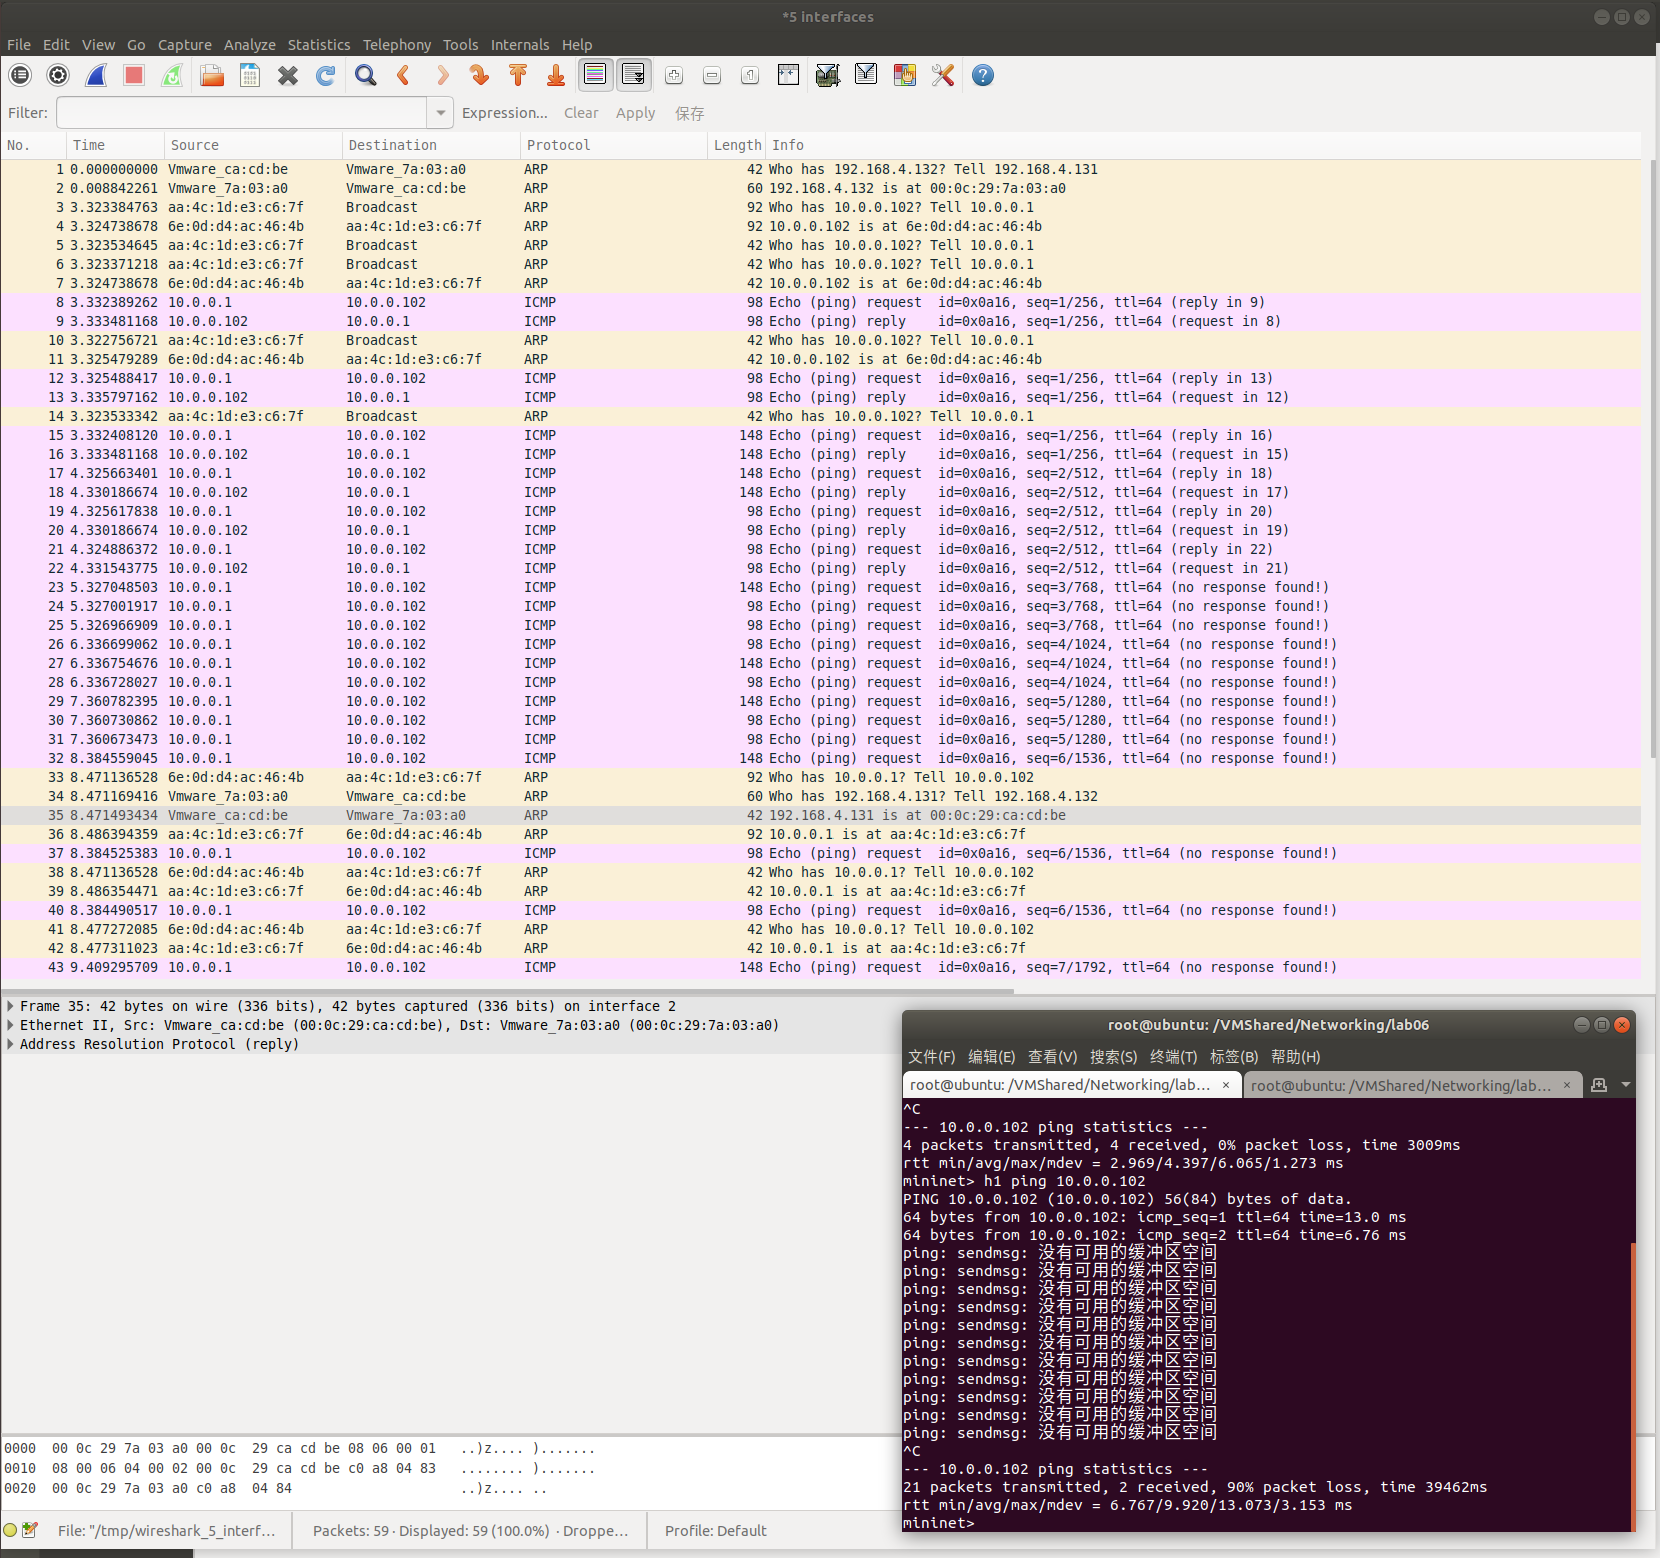
\includegraphics[width=\linewidth]{wiresharkh1ping}
        \caption{无缓冲区空间抓包情况}\label{fig:wiresharkh1ping}
    \end{figure}

    更进一步的测试表明,同一条路径上 \verb"s1-h3",如果是 \verb"s1" 为主动ping方,可以ping通,而如果是 \verb"h3" 为主动方,则ping不通,如图 \ref{fig:pingeachother} 所示。\textbf{疑似子网内的主机无法被 VxLAN 识别以正确发包,或者有机制缺陷,导致只能ping通两次而没有释放缓冲区。}
    
    \begin{figure}[H]
        \centering
        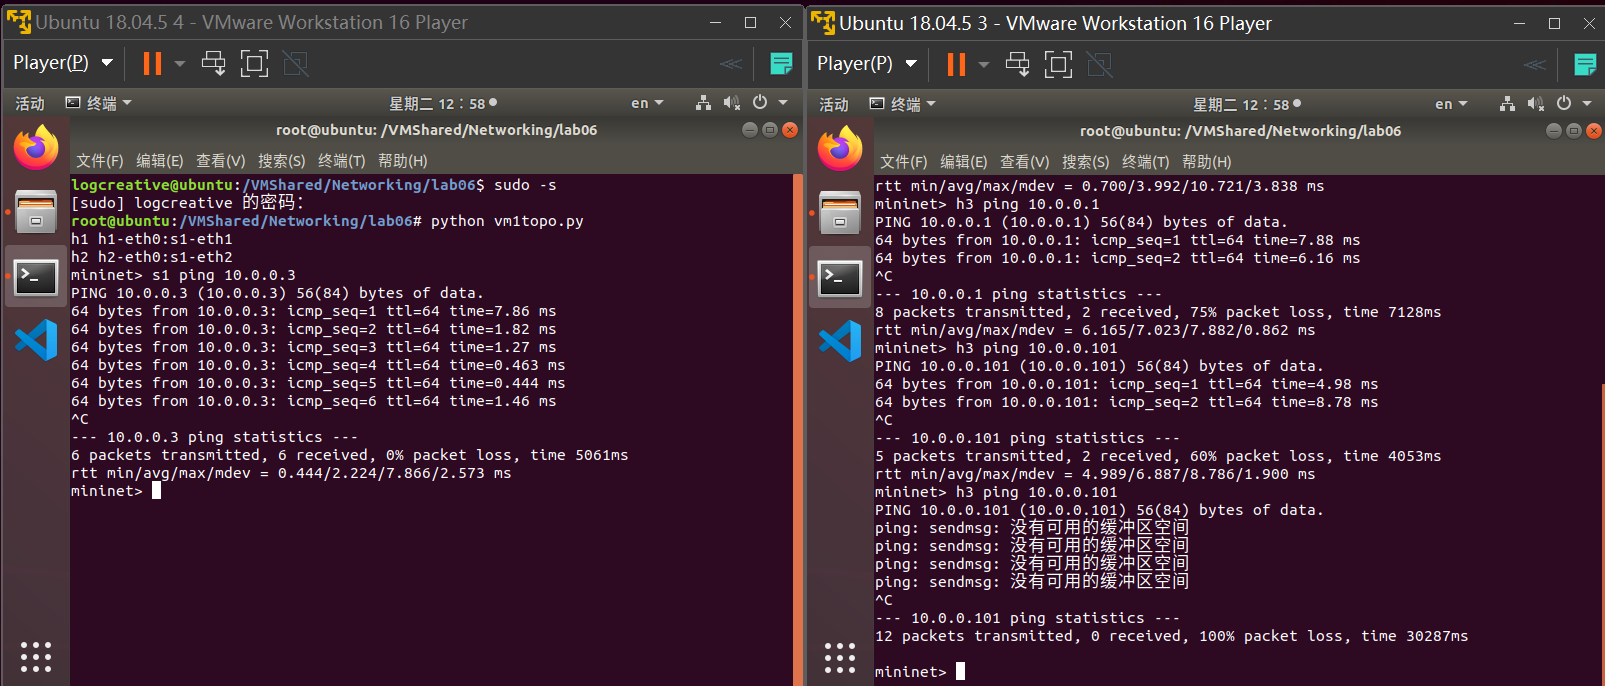
\includegraphics[width=\linewidth]{pingeachother}
        \caption{同一路径不同发送主动方测试}\label{fig:pingeachother}
    \end{figure}

    下面暂时解决方法是直接将服务请求方全部放在交换机上。以及可能会手写控制器\cite{vxlannew}。

    \begin{table}[H]
        \centering
        \caption{运行环境}\label{tab:env}
        \begin{tabular}{>{\bfseries}cl}
            \toprule
            操作系统 & Ubuntu 18.04.5 \\
            虚拟软件 & VMWare Workstation \\
            克隆设置 & 链接克隆与完整克隆皆已测试 \\
            \bottomrule
        \end{tabular}
    \end{table}

    \bibliography{ref}

\end{document}